\begin{sidewaysfigure}[htbp]
\centering 
  \subfloat[Low friction, average void fraction.]
  {
	  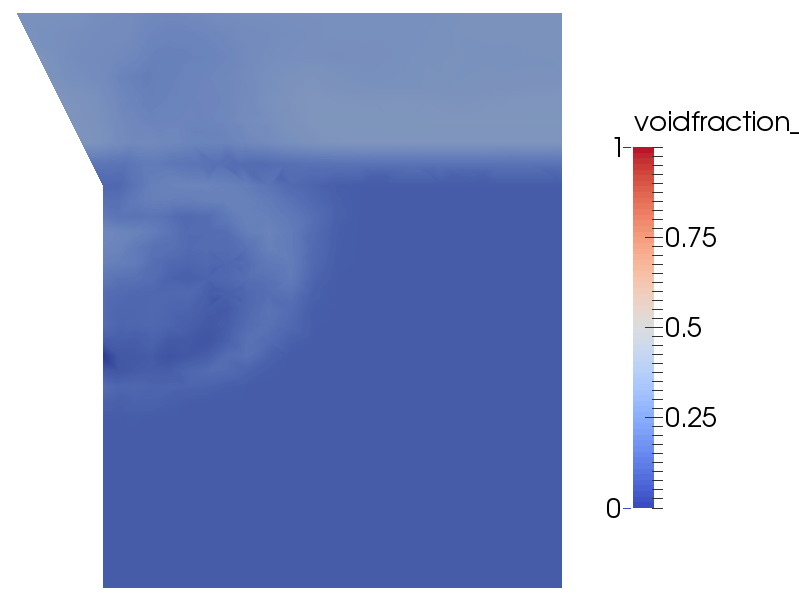
\includegraphics[width=.3\columnwidth]{images/237vf_std_lf}
	  \label{fig:237vf_std_lf}
  }
  \quad
    \subfloat[High friction, average void fraction.]
    {
	  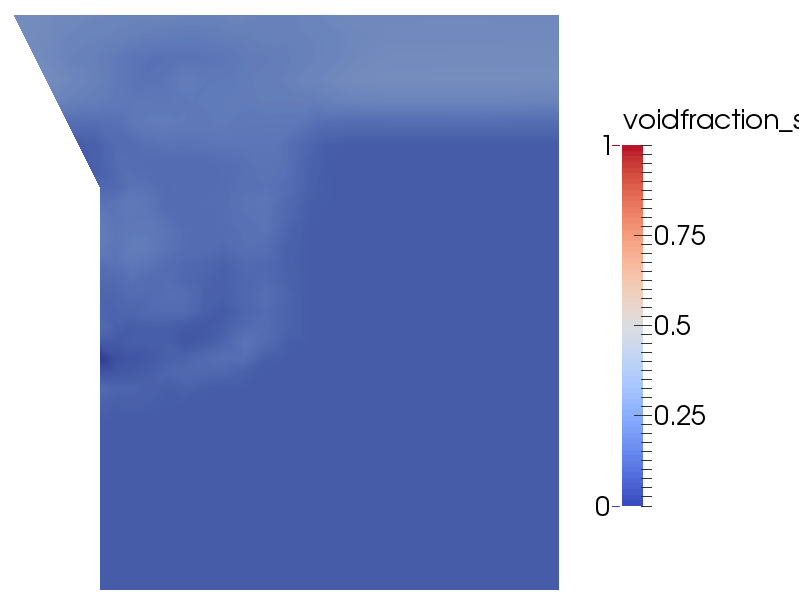
\includegraphics[width=.3\columnwidth]{images/257vf_std_mf}
	  \label{fig:257vf_std_mf}
  }
  \quad
    \subfloat[High friction, average void fraction.]
    {
	  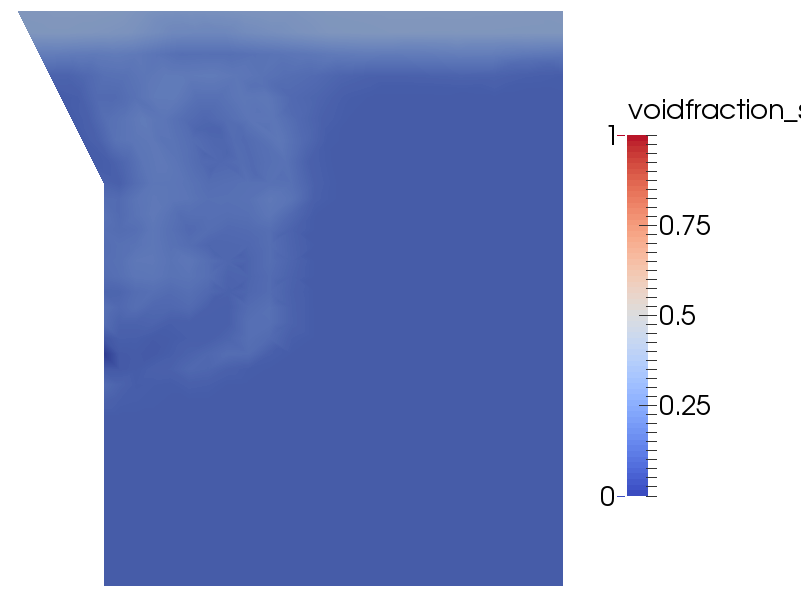
\includegraphics[width=.3\columnwidth]{images/236vf_std_hf}
	  \label{fig:236vf_std_hf}
  }
  \\
  \subfloat[Low friction, standard deviation void fraction.]
  {
	  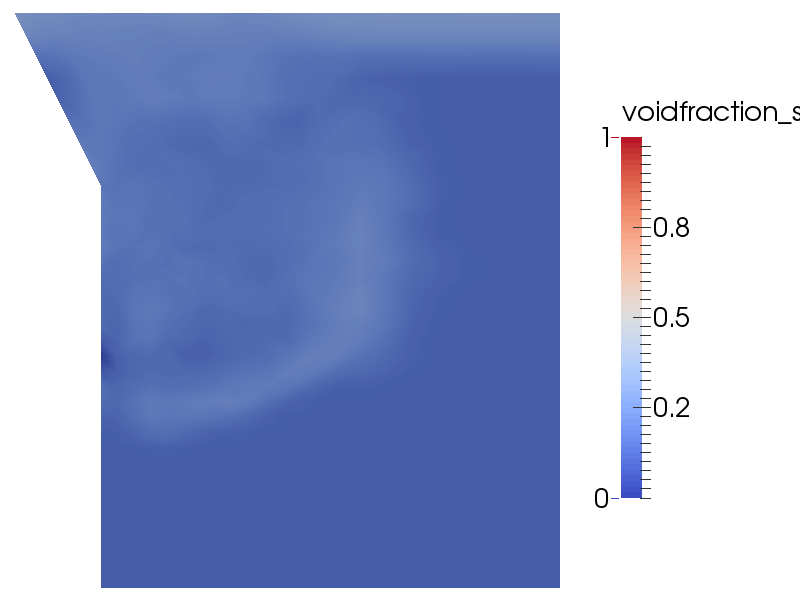
\includegraphics[width=.3\columnwidth]{images/256vf_std_lfhv}
	  \label{fig:256vf_std_lfhv}
  }
  \quad
    \subfloat[High friction, standard deviation void fraction.]
    {
	  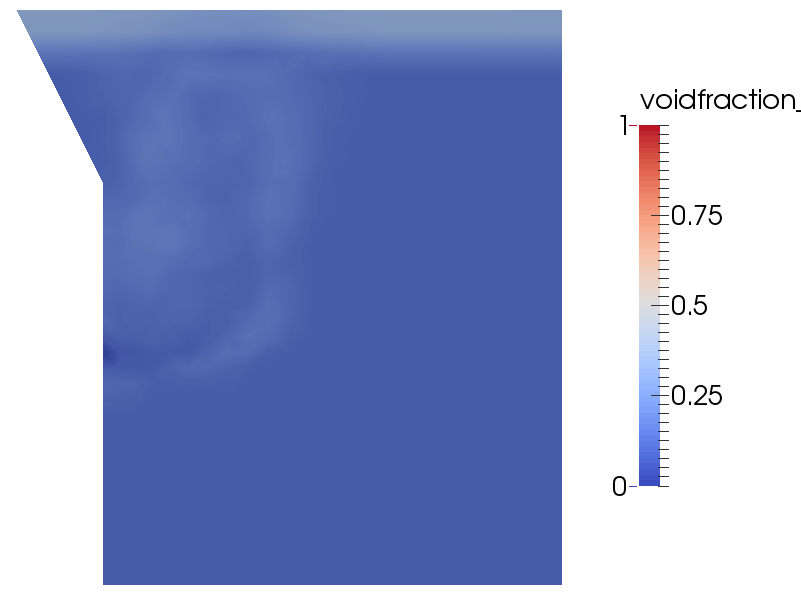
\includegraphics[width=.3\columnwidth]{images/255vf_std_hfhr}
	  \label{fig:255vf_std_hfhr}  }
  \\
  \caption{Standard deviation void fraction with different sliding friction
  coefficient.}
  \label{fig:260racewayvfstd}
\end{sidewaysfigure}